\documentclass{article}
\usepackage{amsmath, amssymb, graphicx, geometry, tikz, array, booktabs, enumitem, listings, xcolor, fancyhdr, float, subcaption, hyperref}

\title{Module 6: Duality in Linear Classification}
\author{Machine Learning Course}
\date{}

\begin{document}

\maketitle
\tableofcontents
\newpage

\section{Introduction to Duality}

\subsection{The Concept of Duality}
In optimization theory, every problem has two perspectives: the primal problem (original formulation) and the dual problem (alternative formulation). Duality is a fundamental concept that provides an alternative way to solve optimization problems, often with significant computational advantages.

\begin{itemize}
    \item \textbf{Primal problem}: The original formulation of the optimization problem
    \item \textbf{Dual problem}: An alternative formulation derived from the primal problem
\end{itemize}

Under certain conditions (particularly for convex optimization problems), the primal and dual problems have the same optimal value, a property known as strong duality.

\subsection{Importance in Machine Learning}
Duality plays a crucial role in machine learning, particularly for linear classification algorithms like the Perceptron and Support Vector Machines (SVMs). The dual formulation:

\begin{itemize}
    \item Provides computational advantages for high-dimensional data
    \item Enables the use of kernel methods for non-linear classification
    \item Offers insights into the structure of the solution
    \item Identifies the most important training examples (support vectors)
\end{itemize}

\section{Dual Form of the Perceptron}

\subsection{Review of the Perceptron Algorithm}
The Perceptron is an algorithm for learning a linear classifier from labeled training data. Given a training set $\{(x^{(i)}, y^{(i)}): i=1,\ldots,n\}$ where $x^{(i)} \in \mathbb{R}^d$ and $y^{(i)} \in \{-1, +1\}$, the Perceptron algorithm works as follows:

\fbox{
\begin{minipage}{\dimexpr\textwidth-2\fboxsep-2\fboxrule\relax}
\textbf{The Perceptron Algorithm}
\begin{enumerate}
    \item Initialize $w = 0$ and $b = 0$
    \item While some training point $(x, y)$ is misclassified:
    \begin{enumerate}
        \item $w = w + yx$
        \item $b = b + y$
    \end{enumerate}
\end{enumerate}
\end{minipage}
}

A point $(x, y)$ is misclassified if $y(w \cdot x + b) \leq 0$, meaning that the predicted label $\text{sign}(w \cdot x + b)$ does not match the true label $y$.

\subsection{Deriving the Dual Representation}
The key insight for the dual form of the Perceptron is that the weight vector $w$ can be expressed as a linear combination of the training examples.

Starting with $w = 0$, each update adds $yx$ to $w$. After multiple updates, $w$ can be written as:

\[
w = \sum_{i=1}^{n} \alpha_i y^{(i)} x^{(i)}
\]

where $\alpha_i$ represents the number of times an update occurred on point $i$.

\begin{figure}[h]
\centering
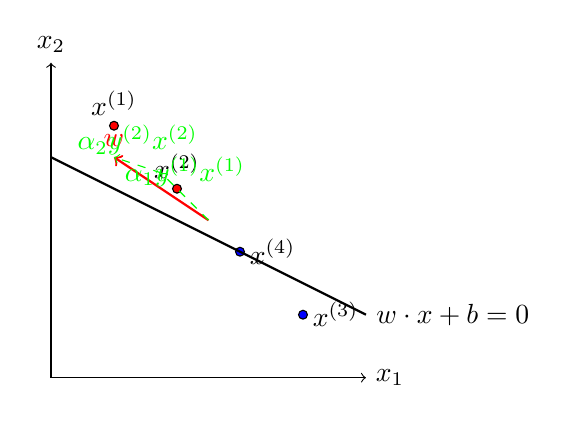
\begin{tikzpicture}[scale=0.8]
    % Coordinate axes
    \draw[->] (0,0) -- (5,0) node[right] {$x_1$};
    \draw[->] (0,0) -- (0,5) node[above] {$x_2$};
    
    % Data points
    \draw[fill=red] (1,4) circle (2pt) node[above] {$x^{(1)}$};
    \draw[fill=red] (2,3) circle (2pt) node[above] {$x^{(2)}$};
    \draw[fill=blue] (4,1) circle (2pt) node[right] {$x^{(3)}$};
    \draw[fill=blue] (3,2) circle (2pt) node[right] {$x^{(4)}$};
    
    % Decision boundary
    \draw[thick, black] (0,3.5) -- (5,1) node[right] {$w \cdot x + b = 0$};
    
    % Weight vector
    \draw[->, thick, red] (2.5,2.5) -- (1,3.5) node[above] {$w$};
    
    % Components
    \draw[->, dashed, green] (2.5,2.5) -- (1.75,3.25) node[midway, above] {$\alpha_1 y^{(1)} x^{(1)}$};
    \draw[->, dashed, green] (1.75,3.25) -- (1,3.5) node[midway, above] {$\alpha_2 y^{(2)} x^{(2)}$};
\end{tikzpicture}
\caption{Illustration of the weight vector $w$ as a linear combination of training examples. The red points have label $+1$ and the blue points have label $-1$.}
\end{figure}

\subsection{Making Predictions in the Dual Form}
Using the dual representation of $w$, the prediction for a new point $x$ becomes:

\begin{align}
\text{sign}(w \cdot x + b) &= \text{sign}\left(\sum_{i=1}^{n} \alpha_i y^{(i)} x^{(i)} \cdot x + b\right) \\
&= \text{sign}\left(\sum_{i=1}^{n} \alpha_i y^{(i)} (x^{(i)} \cdot x) + b\right)
\end{align}

This formulation has a crucial property: to make predictions, we only need to compute inner products between the new point $x$ and the training points $x^{(i)}$. We never need to explicitly compute or store the weight vector $w$.

\subsection{Implications of the Dual Form}
The dual form of the Perceptron has several important implications:

\begin{itemize}
    \item \textbf{Computational efficiency}: For high-dimensional data where $d \gg n$, computing and storing inner products can be more efficient than working with the $d$-dimensional weight vector.
    
    \item \textbf{Kernel trick}: The dual form enables the use of kernel functions to implicitly map data to higher-dimensional spaces without explicitly computing the mapping.
    
    \item \textbf{Interpretability}: The coefficients $\alpha_i$ indicate the importance of each training example in determining the decision boundary.
\end{itemize}

\section{Duality in Optimization}

\subsection{Lagrangian Duality}
Duality in optimization is typically derived using Lagrangian methods. For a constrained optimization problem:

\begin{align}
\min_{x} f(x) \quad \text{subject to} \quad g_i(x) \leq 0, \quad h_j(x) = 0
\end{align}

The Lagrangian function is defined as:

\begin{align}
L(x, \lambda, \nu) = f(x) + \sum_i \lambda_i g_i(x) + \sum_j \nu_j h_j(x)
\end{align}

where $\lambda_i \geq 0$ are the Lagrange multipliers for inequality constraints and $\nu_j$ are the Lagrange multipliers for equality constraints.

\subsection{Primal and Dual Problems}
The primal problem is the original optimization problem. The dual problem is:

\begin{align}
\max_{\lambda \geq 0, \nu} \min_{x} L(x, \lambda, \nu)
\end{align}

Under certain conditions (e.g., when the primal problem is convex and satisfies Slater's condition), strong duality holds, meaning that the optimal values of the primal and dual problems are equal.

\subsection{Advantages of the Dual Problem}
Solving the dual problem instead of the primal can offer several advantages:

\begin{itemize}
    \item The dual problem may have fewer variables or simpler constraints
    \item The dual problem may reveal structure in the solution that is not apparent in the primal
    \item For certain problems, the dual can be solved more efficiently
\end{itemize}

\section{Dual Form of the Support Vector Machine}

\subsection{Primal SVM Formulation}
The primal form of the hard-margin SVM aims to find the maximum-margin linear classifier:

\fbox{
\begin{minipage}{\dimexpr\textwidth-2\fboxsep-2\fboxrule\relax}
\textbf{Primal SVM Optimization Problem}

\begin{align}
\min_{w \in \mathbb{R}^d, b \in \mathbb{R}} & \|w\|^2 \\
\text{subject to: } & y^{(i)}(w \cdot x^{(i)} + b) \geq 1 \quad \text{for all } i = 1, 2, \ldots, n
\end{align}
\end{minipage}
}

This is a convex quadratic optimization problem with linear constraints, which guarantees a unique global minimum.

\subsection{Deriving the Dual SVM}
To derive the dual form of the SVM, we first form the Lagrangian:

\begin{align}
L(w, b, \alpha) = \frac{1}{2}\|w\|^2 - \sum_{i=1}^{n} \alpha_i [y^{(i)}(w \cdot x^{(i)} + b) - 1]
\end{align}

where $\alpha_i \geq 0$ are the Lagrange multipliers.

Taking partial derivatives with respect to $w$ and $b$ and setting them to zero:

\begin{align}
\frac{\partial L}{\partial w} &= w - \sum_{i=1}^{n} \alpha_i y^{(i)} x^{(i)} = 0 \\
\Rightarrow w &= \sum_{i=1}^{n} \alpha_i y^{(i)} x^{(i)}
\end{align}

\begin{align}
\frac{\partial L}{\partial b} &= -\sum_{i=1}^{n} \alpha_i y^{(i)} = 0 \\
\Rightarrow \sum_{i=1}^{n} \alpha_i y^{(i)} &= 0
\end{align}

Substituting these back into the Lagrangian, we get the dual problem:

\fbox{
\begin{minipage}{\dimexpr\textwidth-2\fboxsep-2\fboxrule\relax}
\textbf{Dual SVM Optimization Problem}

\begin{align}
\max_{\alpha \in \mathbb{R}^n} & \sum_{i=1}^{n} \alpha_i - \frac{1}{2} \sum_{i=1}^{n} \sum_{j=1}^{n} \alpha_i \alpha_j y^{(i)} y^{(j)} (x^{(i)} \cdot x^{(j)}) \\
\text{subject to: } & \sum_{i=1}^{n} \alpha_i y^{(i)} = 0 \\
& \alpha_i \geq 0 \quad \text{for all } i = 1, 2, \ldots, n
\end{align}
\end{minipage}
}

\subsection{Making Predictions with the Dual SVM}
Using the dual form, the prediction for a new point $x$ is:

\begin{align}
\text{sign}(w \cdot x + b) &= \text{sign}\left(\sum_{i=1}^{n} \alpha_i y^{(i)} (x^{(i)} \cdot x) + b\right)
\end{align}

As with the Perceptron, we only need to compute inner products between the new point and the training points.

\subsection{Support Vectors}
A key property of the SVM solution is that most of the Lagrange multipliers $\alpha_i$ are zero. The training points with non-zero $\alpha_i$ are called support vectors, and they are the only points that influence the decision boundary.

\begin{figure}[h]
\centering
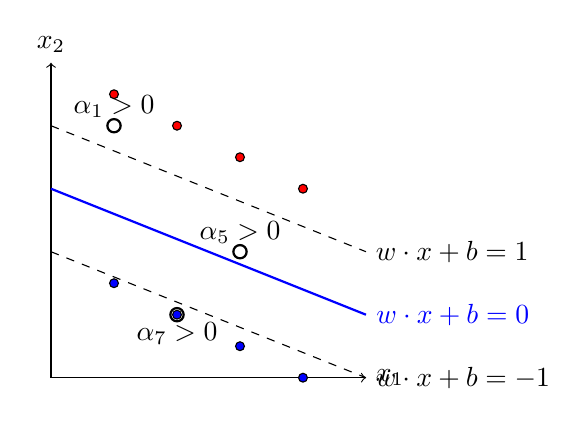
\begin{tikzpicture}[scale=0.8]
    % Coordinate axes
    \draw[->] (0,0) -- (5,0) node[right] {$x_1$};
    \draw[->] (0,0) -- (0,5) node[above] {$x_2$};
    
    % Decision boundary
    \draw[thick, blue] (0,3) -- (5,1) node[right] {$w \cdot x + b = 0$};
    
    % Margin boundaries
    \draw[dashed] (0,4) -- (5,2) node[right] {$w \cdot x + b = 1$};
    \draw[dashed] (0,2) -- (5,0) node[right] {$w \cdot x + b = -1$};
    
    % Data points
    \foreach \x/\y in {1/4.5, 2/4, 3/3.5, 4/3}
        \draw[fill=red] (\x,\y) circle (2pt);
    
    \foreach \x/\y in {1/1.5, 2/1, 3/0.5, 4/0}
        \draw[fill=blue] (\x,\y) circle (2pt);
    
    % Support vectors
    \draw[thick] (1,4) circle (3pt);
    \draw[thick] (3,2) circle (3pt);
    \draw[thick] (2,1) circle (3pt);
    
    % Labels
    \node at (1,4.3) {$\alpha_1 > 0$};
    \node at (3,2.3) {$\alpha_5 > 0$};
    \node at (2,0.7) {$\alpha_7 > 0$};
\end{tikzpicture}
\caption{Illustration of support vectors in an SVM. Only the points on the margin boundaries (circled) have non-zero $\alpha_i$ values and influence the decision boundary.}
\end{figure}

\section{Dual Form of the Soft-Margin SVM}

\subsection{Primal Soft-Margin SVM}
The soft-margin SVM extends the hard-margin SVM to handle non-linearly separable data by introducing slack variables $\xi_i$ that allow for some misclassifications:

\fbox{
\begin{minipage}{\dimexpr\textwidth-2\fboxsep-2\fboxrule\relax}
\textbf{Primal Soft-Margin SVM Optimization Problem}

\begin{align}
\min_{w \in \mathbb{R}^d, b \in \mathbb{R}, \xi \in \mathbb{R}^n} & \|w\|^2 + C \sum_{i=1}^{n} \xi_i \\
\text{subject to: } & y^{(i)}(w \cdot x^{(i)} + b) \geq 1 - \xi_i \quad \text{for all } i = 1, 2, \ldots, n \\
& \xi_i \geq 0 \quad \text{for all } i = 1, 2, \ldots, n
\end{align}
\end{minipage}
}

The parameter $C > 0$ controls the trade-off between maximizing the margin and minimizing the classification error.

\subsection{Dual Soft-Margin SVM}
The dual form of the soft-margin SVM is:

\fbox{
\begin{minipage}{\dimexpr\textwidth-2\fboxsep-2\fboxrule\relax}
\textbf{Dual Soft-Margin SVM Optimization Problem}

\begin{align}
\max_{\alpha \in \mathbb{R}^n} & \sum_{i=1}^{n} \alpha_i - \frac{1}{2} \sum_{i=1}^{n} \sum_{j=1}^{n} \alpha_i \alpha_j y^{(i)} y^{(j)} (x^{(i)} \cdot x^{(j)}) \\
\text{subject to: } & \sum_{i=1}^{n} \alpha_i y^{(i)} = 0 \\
& 0 \leq \alpha_i \leq C \quad \text{for all } i = 1, 2, \ldots, n
\end{align}
\end{minipage}
}

The main difference from the hard-margin dual is the upper bound $C$ on the Lagrange multipliers $\alpha_i$.

\subsection{Interpreting the Dual Variables}
In the soft-margin SVM, the dual variables $\alpha_i$ have the following interpretation:

\begin{itemize}
    \item $\alpha_i = 0$: The point is correctly classified and outside the margin
    \item $0 < \alpha_i < C$: The point is a support vector lying exactly on the margin
    \item $\alpha_i = C$: The point is either misclassified or correctly classified but inside the margin
\end{itemize}

\begin{figure}[h]
\centering
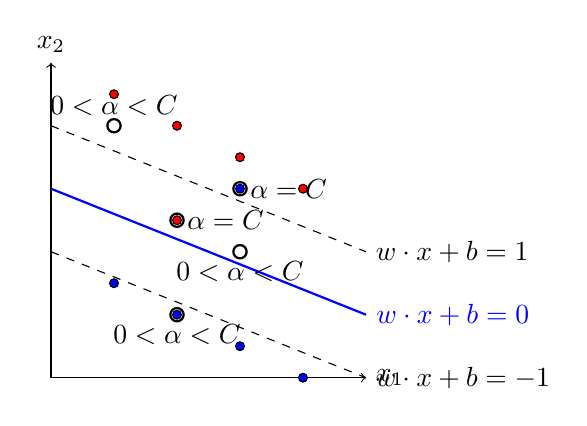
\begin{tikzpicture}[scale=0.8]
    % Coordinate axes
    \draw[->] (0,0) -- (5,0) node[right] {$x_1$};
    \draw[->] (0,0) -- (0,5) node[above] {$x_2$};
    
    % Decision boundary
    \draw[thick, blue] (0,3) -- (5,1) node[right] {$w \cdot x + b = 0$};
    
    % Margin boundaries
    \draw[dashed] (0,4) -- (5,2) node[right] {$w \cdot x + b = 1$};
    \draw[dashed] (0,2) -- (5,0) node[right] {$w \cdot x + b = -1$};
    
    % Data points
    \foreach \x/\y in {1/4.5, 2/4, 3/3.5, 4/3}
        \draw[fill=red] (\x,\y) circle (2pt);
    
    \foreach \x/\y in {1/1.5, 2/1, 3/0.5, 4/0}
        \draw[fill=blue] (\x,\y) circle (2pt);
    
    % Outliers
    \draw[fill=red] (2,2.5) circle (2pt);
    \draw[fill=blue] (3,3) circle (2pt);
    
    % Support vectors
    \draw[thick] (1,4) circle (3pt) node[above] {$0 < \alpha < C$};
    \draw[thick] (3,2) circle (3pt) node[below] {$0 < \alpha < C$};
    \draw[thick] (2,1) circle (3pt) node[below] {$0 < \alpha < C$};
    \draw[thick] (2,2.5) circle (3pt) node[right] {$\alpha = C$};
    \draw[thick] (3,3) circle (3pt) node[right] {$\alpha = C$};
\end{tikzpicture}
\caption{Illustration of support vectors in a soft-margin SVM. Points on the margin have $0 < \alpha_i < C$, while misclassified points or points inside the margin have $\alpha_i = C$.}
\end{figure}

\section{Advantages of the Dual Formulation}

\subsection{Computational Efficiency}
The dual formulation can be more computationally efficient than the primal when:

\begin{itemize}
    \item The number of features $d$ is much larger than the number of training examples $n$
    \item The solution is sparse (few support vectors)
\end{itemize}

In such cases, solving the dual problem and making predictions using only the support vectors can significantly reduce computation and memory requirements.

\subsection{The Kernel Trick}
The most significant advantage of the dual formulation is that it enables the use of the kernel trick. Since both the optimization and prediction only involve inner products between data points, we can replace these inner products with kernel functions:

\begin{align}
K(x^{(i)}, x^{(j)}) = \phi(x^{(i)}) \cdot \phi(x^{(j)})
\end{align}

where $\phi$ is a mapping to a higher-dimensional feature space. This allows SVMs to learn non-linear decision boundaries without explicitly computing the mapping $\phi$.

Common kernel functions include:
\begin{itemize}
    \item Linear kernel: $K(x, z) = x \cdot z$
    \item Polynomial kernel: $K(x, z) = (x \cdot z + c)^d$
    \item Radial basis function (RBF) kernel: $K(x, z) = \exp(-\gamma \|x - z\|^2)$
\end{itemize}

\begin{figure}[h]
\centering
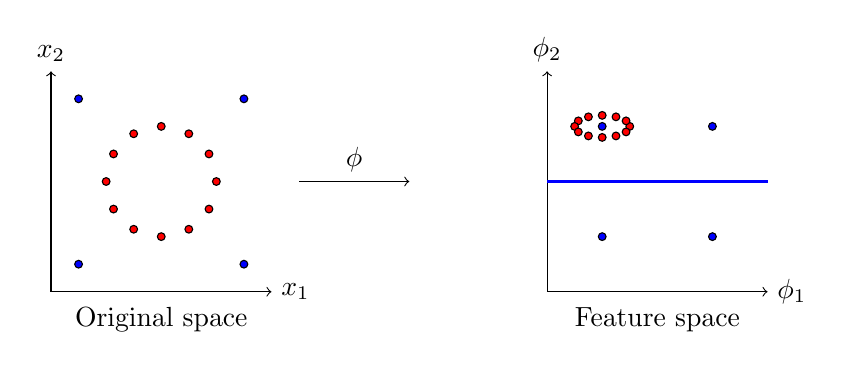
\begin{tikzpicture}[scale=0.7]
    % Original space
    \begin{scope}
        \draw[->] (0,0) -- (4,0) node[right] {$x_1$};
        \draw[->] (0,0) -- (0,4) node[above] {$x_2$};
        
        % Circle of points
        \foreach \angle in {0,30,...,330}
            \draw[fill=red] ({2+cos(\angle)},{2+sin(\angle)}) circle (2pt);
        
        % Outer points
        \foreach \x/\y in {0.5/0.5, 0.5/3.5, 3.5/0.5, 3.5/3.5}
            \draw[fill=blue] (\x,\y) circle (2pt);
        
        \node at (2,-0.5) {Original space};
    \end{scope}
    
    % Arrow
    \draw[->] (4.5,2) -- (6.5,2) node[midway, above] {$\phi$};
    
    % Feature space
    \begin{scope}[xshift=9cm]
        \draw[->] (0,0) -- (4,0) node[right] {$\phi_1$};
        \draw[->] (0,0) -- (0,4) node[above] {$\phi_2$};
        
        % Transformed points
        \foreach \angle in {0,30,...,330}
            \draw[fill=red] ({1+0.5*cos(\angle)},{3+0.2*sin(\angle)}) circle (2pt);
        
        \foreach \x/\y in {3/1, 3/3, 1/1, 1/3}
            \draw[fill=blue] (\x,\y) circle (2pt);
        
        % Linear separator
        \draw[thick, blue] (0,2) -- (4,2);
        
        \node at (2,-0.5) {Feature space};
    \end{scope}
\end{tikzpicture}
\caption{The kernel trick maps data to a higher-dimensional space where it becomes linearly separable.}
\end{figure}

\section{Practical Examples of Dual SVMs}

\subsection{Example 1: Linear Separable Case}
Let's consider a simple 2D example with linearly separable data:
\begin{itemize}
    \item Positive examples: $(1,3)$, $(2,4)$, $(3,3)$
    \item Negative examples: $(1,1)$, $(2,1)$, $(3,2)$
\end{itemize}

\begin{figure}[h]
\centering
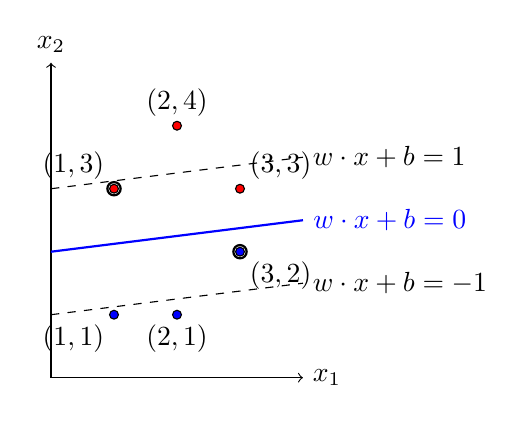
\begin{tikzpicture}[scale=0.8]
    % Coordinate axes
    \draw[->] (0,0) -- (4,0) node[right] {$x_1$};
    \draw[->] (0,0) -- (0,5) node[above] {$x_2$};
    
    % Data points
    \draw[fill=red] (1,3) circle (2pt) node[above left] {$(1,3)$};
    \draw[fill=red] (2,4) circle (2pt) node[above] {$(2,4)$};
    \draw[fill=red] (3,3) circle (2pt) node[above right] {$(3,3)$};
    \draw[fill=blue] (1,1) circle (2pt) node[below left] {$(1,1)$};
    \draw[fill=blue] (2,1) circle (2pt) node[below] {$(2,1)$};
    \draw[fill=blue] (3,2) circle (2pt) node[below right] {$(3,2)$};
    
    % Decision boundary
    \draw[thick, blue] (0,2) -- (4,2.5) node[right] {$w \cdot x + b = 0$};
    
    % Margin boundaries
    \draw[dashed] (0,1) -- (4,1.5) node[right] {$w \cdot x + b = -1$};
    \draw[dashed] (0,3) -- (4,3.5) node[right] {$w \cdot x + b = 1$};
    
    % Support vectors
    \draw[thick] (1,3) circle (3pt);
    \draw[thick] (3,2) circle (3pt);
\end{tikzpicture}
\caption{Example of a linear SVM with support vectors circled}
\end{figure}

Solving the dual SVM optimization problem for this dataset:
\begin{align}
\max_{\alpha} \sum_{i=1}^{6} \alpha_i - \frac{1}{2} \sum_{i=1}^{6} \sum_{j=1}^{6} \alpha_i \alpha_j y^{(i)} y^{(j)} (x^{(i)} \cdot x^{(j)})
\end{align}
subject to $\sum_{i=1}^{6} \alpha_i y^{(i)} = 0$ and $\alpha_i \geq 0$ for all $i$.

The solution would have $\alpha_i > 0$ only for the support vectors (the points on the margin), which in this case are $(1,3)$ and $(3,2)$.

\subsection{Example 2: Non-linear Case with Kernel}
Now, let's consider a dataset that is not linearly separable:
\begin{itemize}
    \item Positive examples: $(1,1)$, $(2,2)$, $(3,1)$
    \item Negative examples: $(1,2)$, $(2,1)$, $(3,2)$
\end{itemize}

\begin{figure}[h]
\centering
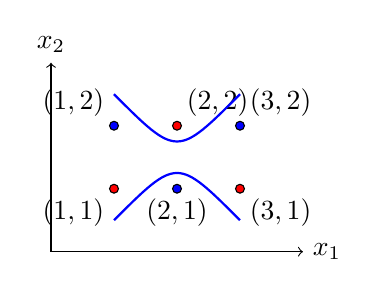
\begin{tikzpicture}[scale=0.8]
    % Coordinate axes
    \draw[->] (0,0) -- (4,0) node[right] {$x_1$};
    \draw[->] (0,0) -- (0,3) node[above] {$x_2$};
    
    % Data points
    \draw[fill=red] (1,1) circle (2pt) node[below left] {$(1,1)$};
    \draw[fill=red] (2,2) circle (2pt) node[above right] {$(2,2)$};
    \draw[fill=red] (3,1) circle (2pt) node[below right] {$(3,1)$};
    \draw[fill=blue] (1,2) circle (2pt) node[above left] {$(1,2)$};
    \draw[fill=blue] (2,1) circle (2pt) node[below] {$(2,1)$};
    \draw[fill=blue] (3,2) circle (2pt) node[above right] {$(3,2)$};
    
    % Non-linear decision boundary
    \draw[thick, blue] (1,0.5) .. controls (2,1.5) .. (3,0.5);
    \draw[thick, blue] (1,2.5) .. controls (2,1.5) .. (3,2.5);
\end{tikzpicture}
\caption{Example of a non-linear classification problem}
\end{figure}

This dataset is not linearly separable, but we can use a kernel function to map the data to a higher-dimensional space where it becomes separable. Using a polynomial kernel $K(x, z) = (x \cdot z + 1)^2$, the dual optimization problem becomes:
\begin{align}
\max_{\alpha} \sum_{i=1}^{6} \alpha_i - \frac{1}{2} \sum_{i=1}^{6} \sum_{j=1}^{6} \alpha_i \alpha_j y^{(i)} y^{(j)} K(x^{(i)}, x^{(j)})
\end{align}
subject to $\sum_{i=1}^{6} \alpha_i y^{(i)} = 0$ and $0 \leq \alpha_i \leq C$ for all $i$.

The decision boundary in the original space would be non-linear, as shown in the figure.

\section{Implementing Dual SVMs}

\subsection{Solving the Dual Optimization Problem}
The dual SVM optimization problem is a quadratic programming (QP) problem, which can be solved using standard QP solvers. Here's a high-level approach:

\begin{enumerate}
    \item Compute the Gram matrix $G$ where $G_{ij} = y^{(i)} y^{(j)} K(x^{(i)}, x^{(j)})$
    \item Solve the QP problem to find the optimal $\alpha$
    \item Identify the support vectors (points with $\alpha_i > 0$)
    \item Compute the bias term $b$
\end{enumerate}

\subsection{Computing the Bias Term}
For any support vector $x^{(s)}$ with $0 < \alpha_s < C$, the bias term $b$ can be computed as:
\begin{align}
b = y^{(s)} - \sum_{i=1}^{n} \alpha_i y^{(i)} K(x^{(i)}, x^{(s)})
\end{align}

It's common practice to average the $b$ values computed from multiple support vectors to improve numerical stability.

\subsection{Making Predictions}
Once we have the optimal $\alpha$ and $b$, predictions for new points can be made using:
\begin{align}
\text{sign}\left(\sum_{i=1}^{n} \alpha_i y^{(i)} K(x^{(i)}, x) + b\right)
\end{align}

Note that we only need to compute kernel evaluations between the new point $x$ and the support vectors (points with $\alpha_i > 0$).

\subsection{Pseudocode for Dual SVM Implementation}
\fbox{
\begin{minipage}{\dimexpr\textwidth-2\fboxsep-2\fboxrule\relax}
\textbf{Dual SVM Training Algorithm}
\begin{enumerate}
    \item \textbf{Input}: Training data $\{(x^{(i)}, y^{(i)}): i=1,\ldots,n\}$, kernel function $K$, regularization parameter $C$
    \item \textbf{Compute} the Gram matrix $G$ where $G_{ij} = y^{(i)} y^{(j)} K(x^{(i)}, x^{(j)})$
    \item \textbf{Solve} the quadratic programming problem:
    \begin{align}
    \max_{\alpha} \sum_{i=1}^{n} \alpha_i - \frac{1}{2} \sum_{i=1}^{n} \sum_{j=1}^{n} \alpha_i \alpha_j G_{ij}
    \end{align}
    subject to $\sum_{i=1}^{n} \alpha_i y^{(i)} = 0$ and $0 \leq \alpha_i \leq C$ for all $i$
    \item \textbf{Identify} the support vectors $S = \{i: \alpha_i > 0\}$
    \item \textbf{Compute} the bias term $b$:
    \begin{align}
    b = \frac{1}{|S_m|} \sum_{s \in S_m} \left(y^{(s)} - \sum_{i \in S} \alpha_i y^{(i)} K(x^{(i)}, x^{(s)})\right)
    \end{align}
    where $S_m = \{i: 0 < \alpha_i < C\}$ are the margin support vectors
    \item \textbf{Output}: Support vectors, their coefficients $\alpha_i$, and the bias term $b$
\end{enumerate}
\end{minipage}
}

\fbox{
\begin{minipage}{\dimexpr\textwidth-2\fboxsep-2\fboxrule\relax}
\textbf{Dual SVM Prediction Algorithm}
\begin{enumerate}
    \item \textbf{Input}: New point $x$, support vectors $\{x^{(i)}: i \in S\}$, coefficients $\{\alpha_i: i \in S\}$, labels $\{y^{(i)}: i \in S\}$, bias term $b$, kernel function $K$
    \item \textbf{Compute} the decision function:
    \begin{align}
    f(x) = \sum_{i \in S} \alpha_i y^{(i)} K(x^{(i)}, x) + b
    \end{align}
    \item \textbf{Output}: Predicted label $\text{sign}(f(x))$
\end{enumerate}
\end{minipage}
}

\section{Connections to Other Methods}

\subsection{Relationship to Kernel Methods}
The dual formulation of SVMs is closely related to other kernel methods in machine learning:

\begin{itemize}
    \item \textbf{Kernel PCA}: Uses kernels to perform non-linear dimensionality reduction
    \item \textbf{Kernel k-means}: Applies kernels to perform non-linear clustering
    \item \textbf{Gaussian Processes}: Bayesian approach to kernel-based learning
\end{itemize}

All these methods leverage the kernel trick to implicitly work in high-dimensional feature spaces without explicitly computing the mapping.

\subsection{Connection to Neural Networks}
SVMs and neural networks have interesting connections:

\begin{itemize}
    \item Both can learn non-linear decision boundaries
    \item SVMs with certain kernels can be viewed as infinite-width neural networks
    \item The margin concept in SVMs has influenced the design of neural network architectures and training algorithms
\end{itemize}

\subsection{Relationship to Regularized Empirical Risk Minimization}
SVMs can be viewed as a special case of regularized empirical risk minimization:

\begin{itemize}
    \item The objective function $\|w\|^2$ serves as a regularization term
    \item The constraints $y^{(i)}(w \cdot x^{(i)} + b) \geq 1$ correspond to a hinge loss function
    \item The parameter $C$ in soft-margin SVMs controls the trade-off between regularization and empirical risk
\end{itemize}

\section{Advanced Topics in Duality}

\subsection{Karush-Kuhn-Tucker (KKT) Conditions}
The KKT conditions provide necessary conditions for optimality in constrained optimization problems. For the SVM problem, the KKT conditions include:

\begin{itemize}
    \item Stationarity: $w = \sum_{i=1}^{n} \alpha_i y^{(i)} x^{(i)}$
    \item Complementary slackness: $\alpha_i (y^{(i)}(w \cdot x^{(i)} + b) - 1) = 0$ for all $i$
    \item Primal feasibility: $y^{(i)}(w \cdot x^{(i)} + b) \geq 1$ for all $i$
    \item Dual feasibility: $\alpha_i \geq 0$ for all $i$
\end{itemize}

These conditions provide insights into the structure of the SVM solution, particularly the role of support vectors.

\subsection{Sequential Minimal Optimization (SMO)}
SMO is an efficient algorithm for solving the dual SVM optimization problem, especially for large datasets. The key idea is to:

\begin{itemize}
    \item Decompose the large QP problem into a series of smaller QP problems
    \item At each step, optimize only two $\alpha_i$ values while keeping the others fixed
    \item Update the bias term after each optimization step
\end{itemize}

This approach is much more memory-efficient than standard QP solvers and is the basis for many practical SVM implementations.

\subsection{Multi-class SVMs}
SVMs are inherently binary classifiers, but they can be extended to multi-class problems using several strategies:

\begin{itemize}
    \item \textbf{One-vs-Rest}: Train $k$ binary SVMs, each separating one class from the rest
    \item \textbf{One-vs-One}: Train $\binom{k}{2}$ binary SVMs, one for each pair of classes
    \item \textbf{Direct Multi-class Formulation}: Extend the SVM optimization problem to directly handle multiple classes
\end{itemize}

The dual formulation plays a crucial role in all these approaches, particularly for implementing kernel-based multi-class SVMs.

\section{Summary and Key Takeaways}

\subsection{Importance of Duality in Linear Classification}
Duality provides a powerful alternative perspective on linear classification algorithms:

\begin{itemize}
    \item It expresses the weight vector as a linear combination of training examples
    \item It enables the use of kernel methods for non-linear classification
    \item It identifies the most important training examples (support vectors)
    \item It often leads to more efficient algorithms, especially for high-dimensional data
\end{itemize}

\subsection{Dual Form of the Perceptron}
The dual form of the Perceptron:

\begin{itemize}
    \item Expresses the weight vector as $w = \sum_{i} \alpha_i y^{(i)} x^{(i)}$
    \item Makes predictions using inner products: $\text{sign}(\sum_{i} \alpha_i y^{(i)} (x^{(i)} \cdot x) + b)$
    \item Enables the use of kernels for non-linear classification
\end{itemize}

\subsection{Dual Form of the SVM}
The dual form of the SVM:

\begin{itemize}
    \item Transforms the primal minimization problem into a dual maximization problem
    \item Expresses the solution in terms of support vectors
    \item Enables efficient implementation through kernel methods
    \item Provides insights into the structure of the solution
\end{itemize}

\subsection{Practical Implications}
The dual formulation has significant practical implications:

\begin{itemize}
    \item For high-dimensional data, the dual form can be more computationally efficient
    \item The sparsity of the solution (few support vectors) leads to efficient prediction
    \item Kernel methods enable SVMs to learn complex non-linear decision boundaries
    \item The dual form is the basis for many practical SVM implementations
\end{itemize}

\subsection{Future Directions}
Duality continues to play an important role in machine learning research:

\begin{itemize}
    \item Development of more efficient algorithms for solving the dual optimization problem
    \item Exploration of new kernel functions for specific applications
    \item Integration of dual methods with deep learning approaches
    \item Application of duality concepts to other machine learning problems
\end{itemize}

\end{document}on of duality concepts to other machine learning problems
\end{itemize}

\end{document}